% Document setup
\documentclass[12pt]{article}
\usepackage[margin=1in]{geometry}
\usepackage{fancyhdr}
\usepackage{lastpage}

\pagestyle{fancy}
\lhead{Richard Whitehill}
\chead{PHYS 804 -- HW \HWnum}
\rhead{\duedate}
\cfoot{\thepage \hspace{1pt} of \pageref{LastPage}}

% Encoding
\usepackage[utf8]{inputenc}
\usepackage[T1]{fontenc}

% Math/Physics Packages
\usepackage{amsmath}
\usepackage{amssymb}
\usepackage{mathtools}
\usepackage{physics}
\usepackage{siunitx}

\AtBeginDocument{\RenewCommandCopy\qty\SI}

% Enumeration/itemize
\usepackage{enumitem}
\newenvironment{parts}
{\begin{enumerate}[label=\textbf{(\alph*)},leftmargin=*,itemsep=-10pt]
}{\end{enumerate}}

% Reference Style
\usepackage{hyperref}
\hypersetup{
    colorlinks=true,
    linkcolor=blue,
    filecolor=magenta,
    urlcolor=cyan,
    citecolor=green
}

\newcommand{\eref}[1]{Eq.~(\ref{eq:#1})}
\newcommand{\erefs}[2]{Eqs.~(\ref{eq:#1})--(\ref{eq:#2})}

\newcommand{\fref}[1]{Fig.~\ref{fig:#1}}
\newcommand{\frefs}[2]{Figs.~\ref{fig:#1}--\ref{fig:#2}}

\newcommand{\tref}[1]{Table~\ref{tab:#1}}
\newcommand{\trefs}[2]{Tables~\ref{tab:#1}-\ref{tab:#2}}

% Figures and Tables 
\usepackage{graphicx}
\usepackage{float}
\usepackage[font=small,labelfont=bf]{caption}

\newcommand{\bef}{\begin{figure}[h!]\begin{center}}
\newcommand{\eef}{\end{center}\end{figure}}

\newcommand{\bet}{\begin{table}[h!]\begin{center}}
\newcommand{\eet}{\end{center}\end{table}}

% tikz
\usepackage{tikz}
\usetikzlibrary{calc}
\usetikzlibrary{decorations.pathmorphing}
\usetikzlibrary{decorations.markings}
\usetikzlibrary{arrows.meta}
\usetikzlibrary{positioning}
\usetikzlibrary{3d}
\usetikzlibrary{shapes.geometric}

% tcolorbox
\usepackage[most]{tcolorbox}
\usepackage{xcolor}
\usepackage{xifthen}
\usepackage{parskip}

\newcommand*{\eqbox}{\tcboxmath[
    enhanced,
    colback=black!10!white,
    colframe=black,
    sharp corners,
    size=fbox,
    boxsep=8pt,
    boxrule=1pt
]}

% problem-solution macros
% \usepackage{adjustbox}
\usepackage{changepage}

\newtcolorbox{probbox}[1][]{
    breakable,
    enhanced,
    boxrule=0pt,
    frame hidden,
    borderline west={4pt}{0pt}{green!50!black},
    colback=green!5,
    before upper=\textbf{Problem #1) \,},
    % \textbf{Problem #1 \ifthenelse{\isempty{#1}}{}{: #1} \\ },
    sharp corners,
    parbox=false
}

% \newtcolorbox{ProblemBox}[1][]{%
%   breakable,
%   enhanced,
%   colback=black!10!white,
%   colframe=black,
%   title={\large #1 \hfill}
% }
\newcommand{\prob}[2]{
\begin{probbox}[#1]
#2
\end{probbox}
}

\newenvironment{solution}{\begin{adjustwidth}{8pt}{8pt}}{\end{adjustwidth}}
\newcommand{\sol}[1]{
\begin{solution}
#1
\end{solution}
}
% \textbf{#1)} #2}

% Miscellaneous Definitions/Settings
\newcommand{\reals}{\mathbb{R}}
\newcommand{\integers}{\mathbb{Z}}
\newcommand{\naturals}{\mathbb{N}}
\newcommand{\rationals}{\mathbb{Q}}
\newcommand{\complexs}{\mathbb{C}}

\setlength{\parskip}{\baselineskip}
\setlength{\parindent}{0pt}
\setlength{\headheight}{14.49998pt}
\addtolength{\topmargin}{-2.49998pt}


\def\HWnum{2}
\def\duedate{September 17, 2024}

\usepackage{subcaption}


\begin{document}


\prob{1}{

Exploring RNGs:

\begin{parts}

    \item Master using a random number generator available for you.
        Your preference should go, if possible, with the Mersenne Twister generator.

    \item Calculate $5^{\rm th}$ moment of the random number distribution and compare with the expected value.
        Explore how your agreement with the expected value changes as you increase the number of generated random numbers.

    \item Calculate the near-neighbor correlation for $(x_{i},x_{i+5})$ and compare with the expected analytical value.
    
\end{parts}

}

\sol{


(a) For the purposes of this assignment, I use the default random number generator provided by the \textit{numpy} package.
A couple plots using the generator are shown in \fref{prob1_tests}.
Observe that this generator produces a fairly high quality sample of a uniform distribution without a visually obvious correlation between nearby sequence members.

\begin{figure}[h!]
    \centering
    \begin{subfigure}{0.5\textwidth}
        \centering
        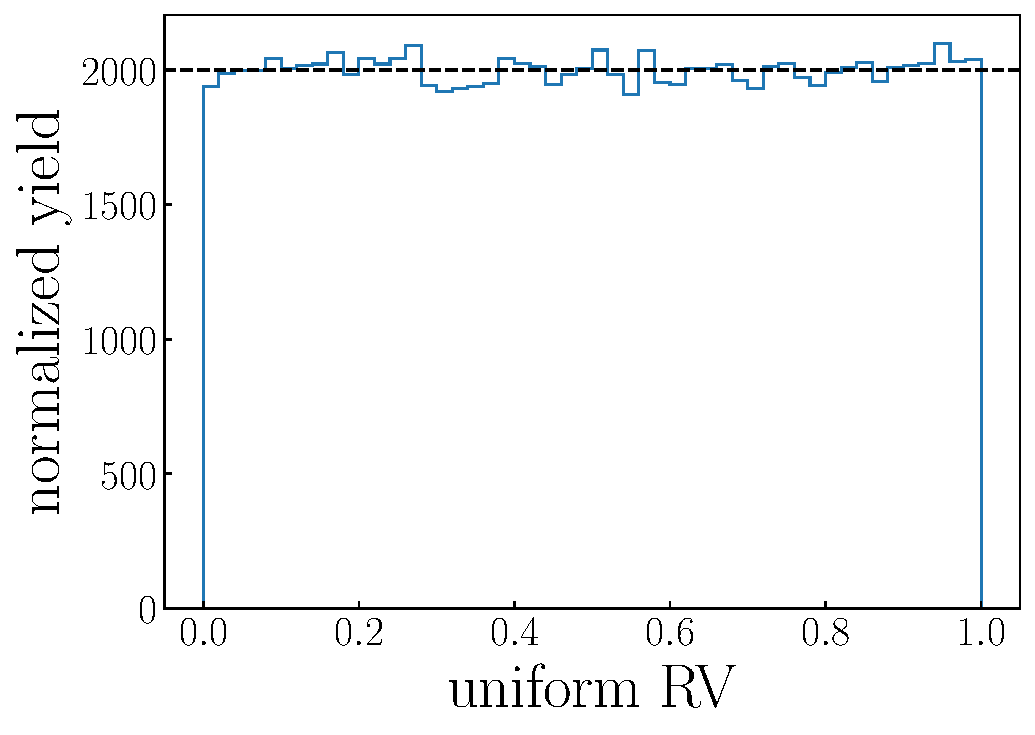
\includegraphics[width=0.8\linewidth]{prob1_uniformity.pdf}
        \caption{}
        \label{fig:prob1_tests-a}
    \end{subfigure}%
    \begin{subfigure}{0.5\textwidth}
        \centering
        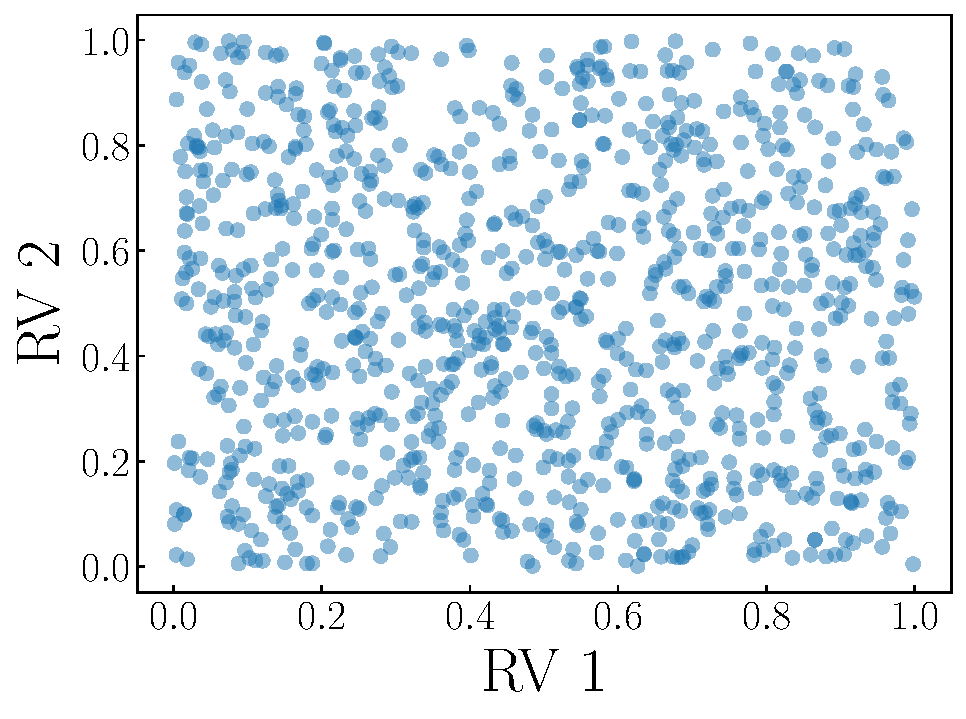
\includegraphics[width=0.8\linewidth]{prob1_parking-lot.pdf}
        \caption{}
        \label{fig:prob1_tests-b}
    \end{subfigure}%
    \caption{\textbf{(a)} -- Uniformity test for random number generator with $10^{6}$ samples. \textbf{(b)} -- Parking lot test for correlation between samples with $10^{3}$ samples for each sequence.}
    \label{fig:prob1_tests}
\end{figure}


(b--c) Using the sample from the random number generator described in part (a), we can calculate the $n^{\rm th}$ moment and near-neighbor correlation between $x_{i}$ and $x_{i+k}$ as
\begin{align}
    \expval{x^{n}} &= \frac{1}{N} \sum_{i=0}^{N} x_{i}^{n} \\
    \expval{x_{i} x_{i+5}} &= \frac{1}{N} \sum_{i=0}^{N-k} x_{i} x_{i+k}
,\end{align}
respectively.
Note that the expected values of such moments and correlations for samples pulled from a uniform distribution are
\begin{align}
    E[x^{n}] &= \int_{0}^{1} \dd{x} x^{n} = \frac{1}{n+1} \\
    E[x_{i} x_{i+k}] &= \int_{0}^{1} \dd{x_1} \int_{0}^{1} \dd{x_2} x_{1} x_{2} = \frac{1}{4}
.\end{align}
From the plots, we can see that as the sample size becomes larger, we approach the random number generator produces fifth moment and correlation values close to the expected values with only a small amount of noise.

\begin{figure}[h!]
    \centering
    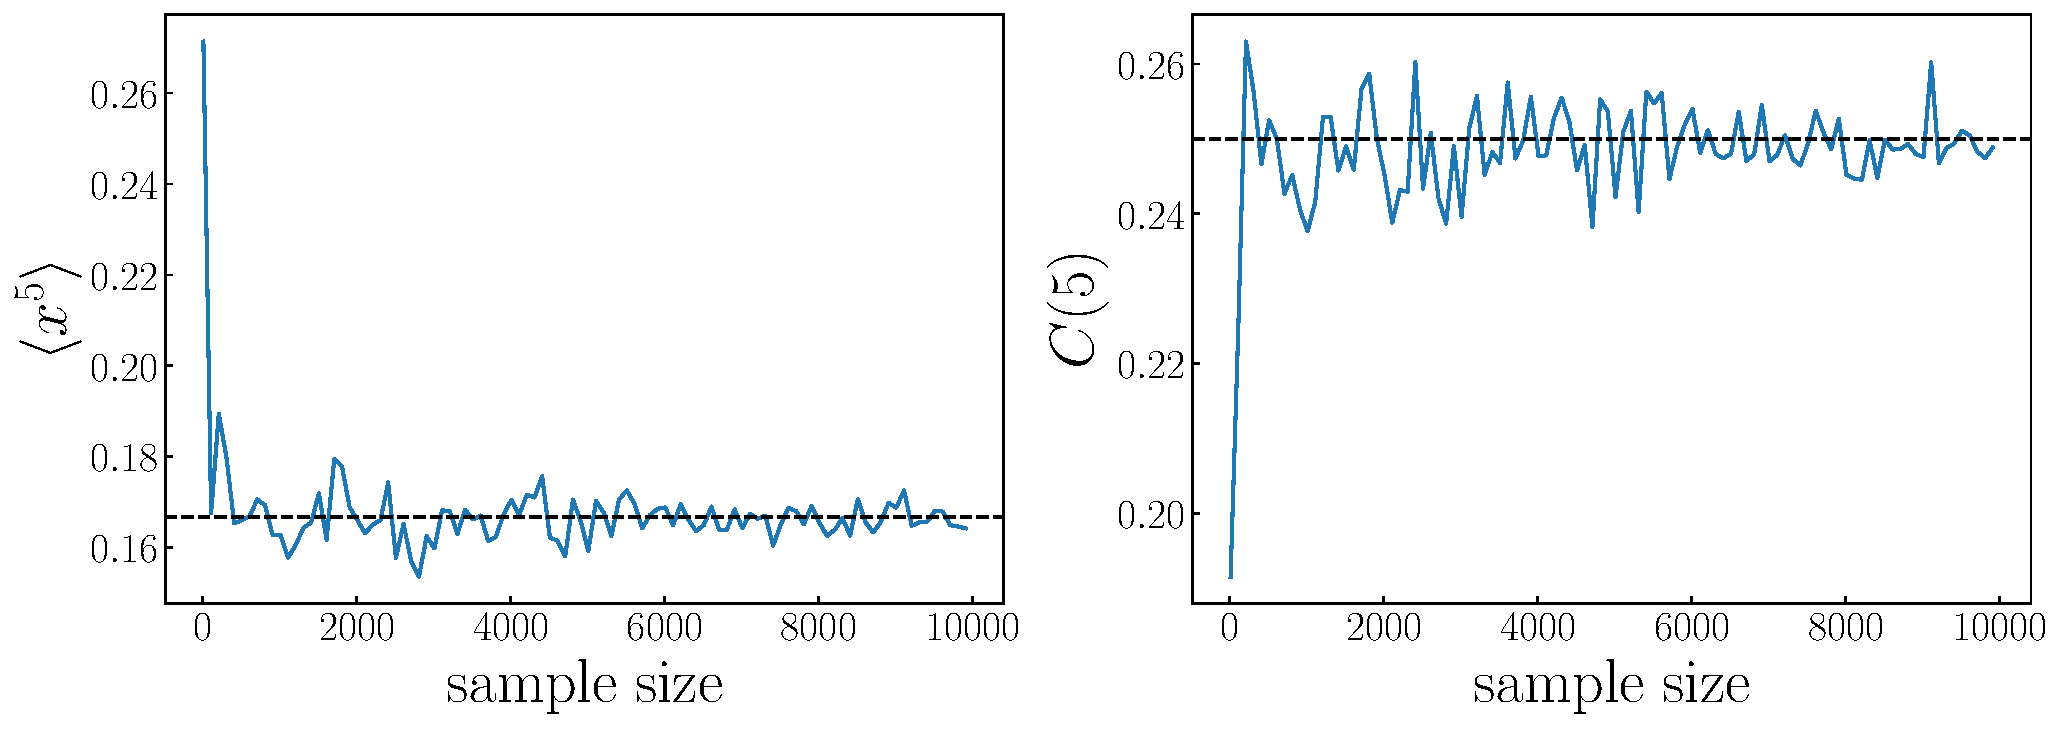
\includegraphics[width=\textwidth]{prob1_mom_corr.pdf}
    \caption{\textbf{Left} -- Fifth moment of a sample of a uniform random variable. Note the dashed black line indicates the expected value, assuming such a uniform distribution. \textbf{Right} -- Near-neighbor correlation between $x_{i}$ and $x_{i+5}$ for the same sample of a uniform random variable. Again, the dashed black line indicates the expected value.}
    \label{fig:prob1_mom-corr}
\end{figure}

\inputpython{exploring_rngs.py}

}


\prob{2}{

Generating non-uniform distribution:

\begin{parts}

    \item Write a code that can generate non-uniform distributions of random numbers based on one, or two or all three of the methods, namely, the rejection method, the transformation method (when possible), and the Metropolis algorithm (importance sampling)

    \item Use your code to generate the following non-uniform distributions:
        \begin{enumerate}
            \item $p(y) = \frac{1}{a} \exp(-y/a)$  (Poisson distribution)

            \item $p(y) = \frac{1}{\pi} \frac{a}{a^2 + y^2}$ (Cauchy-Lorentz distribution)

            \item $p(y) = \frac{1}{\sigma \sqrt{2 \pi}} \exp(-\frac{1}{2}(\frac{y- \mu}{\sigma})^2)$
        \end{enumerate}

    \item Analyze the quality of your distributions in any way you find appropriate.

    \item Explore if any of of the above distributions are available to you with either C++, or Python, or MatLab libraries.

\end{parts}

}

\sol{


(a) A script which implements the transform, rejection, and Metropolis sampling algorithms is shown below.
The transform method is simply implemented when the inverse CDF, $F^{-1}(x;\vb*{a})$ (where $\vb*{a}$ are distribution parameters), of a random variable is known.
Since the output of a CDF is between 0 and 1, we can sample a uniform random variable $u$ and construct the desired random variable $x$ via
\begin{align}
    x = F^{-1}(u;\vb*{a})
.\end{align}
Of course, there are other numerical schemes we can implement to approximate the inverse CDF.
For example, we can solve the problem
\begin{align}
    u = \int_{-\infty}^{x} \dd{t} f(t;\vb*{a})
\end{align}
directly, where $u$ is the sampled uniform random variable, and $x$ is the desired random variable distributed according to the density $f(x;\vb*{a})$.
However, because in most cases, we require a numerical scheme to compute the integral and find the root $x$ corresponding to $u$, such an approach is not always more efficient than other more direct methods of sampling the PDF.

For the rejection method, we uniformly sample points $(x,y) \in [a,b] \times [c,d]$ and keep the sample if $|y| < |f(x;\vb*{a})|$.

Lastly, for the Metropolis algorithm, we choose a starting point $x_0$ and iterate according to the recursive formula
\begin{align}
    x_{i+1} = x_{i} + \delta (2 u - 1)
,\end{align}
where $u \in [0,1]$ is uniformly sampled.
This point is added to the sample if \\ $f(x_{i+1};\vb*{a}) / f(x_{i};\vb*{a}) \geq v$, where $v \in [0,1]$ is uniformly sampled, and the process is repeated until the desired number of samples is achieved.

\inputpython{prob2.py}


(b) In \fref{prob2}, we show samples of the Poisson, Cauchy-Lorentz, and Gaussian distributions are shown.
The following list details the precise setups used to produce the samples.

\begin{itemize}

    \item Poisson:
    \begin{itemize}
       
        \item Rejection: sample on $[0,10] \times [0,1]$ with a rejection rate of $90\%$
        \item Metropolis: sample with starting point $x_0 = 1$ with a step size of $\delta = 0.1$ resulting in a rejection rate of $5\%$

    \end{itemize}

    \item Cauchy-Lorentz:
    \begin{itemize}
       
        \item Rejection: sample on $[-10,10] \times [0,1/\pi]$ with a rejection rate of $85\%$
        \item Metropolis: sample with starting point $x_0 = 0$ with a step size of $\delta = 1$ resulting in a rejection rate of $18\%$

    \end{itemize}

    \item Gaussian:
    \begin{itemize}
       
        \item Rejection: sample on $[-10,10] \times [0,1/\sqrt{2 \pi}]$ with a rejection rate of $88\%$
        \item Metropolis: sample with starting point $x_0 = 0$ with a step size of $\delta = 1$ resulting in a rejection rate of $25\%$

    \end{itemize}


    
\end{itemize}



\begin{figure}[h!]
    \centering
    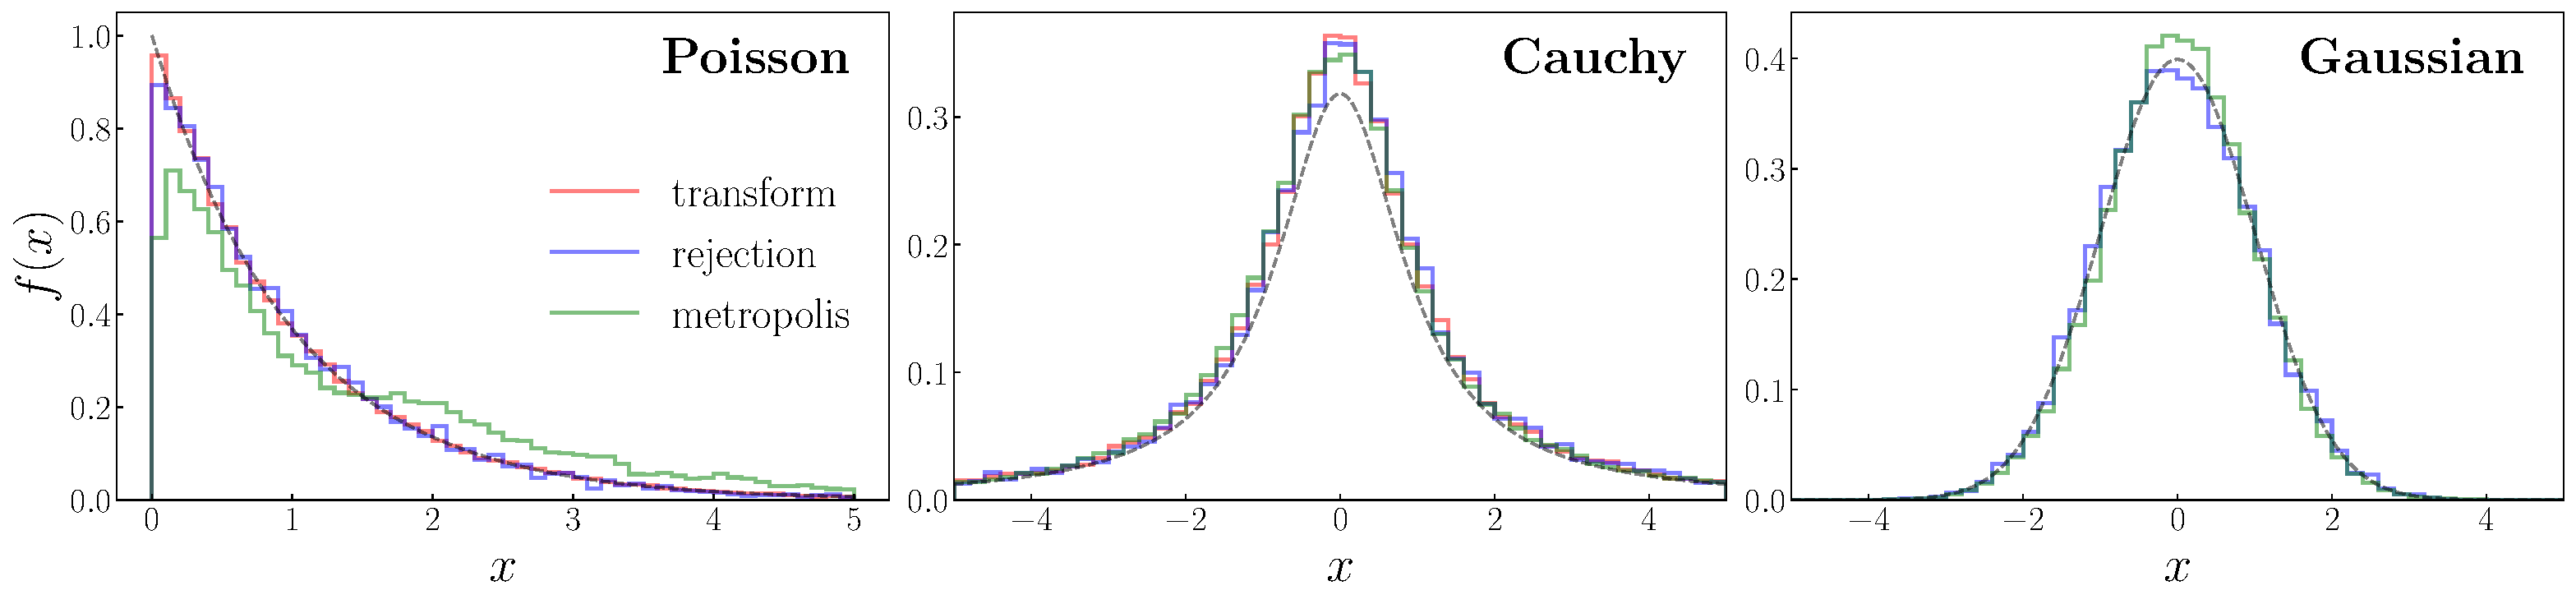
\includegraphics[width=\textwidth]{prob2.pdf}
    \caption{Samples ($N = 10^{5}$), collected into histograms with 50 bins across the selected ranges, for the Poisson ($a = 1$), Cauchy-Lorentz ($a = 1$), and Gaussian probability distributions ($\mu = 0, \sigma = 1$). Note that we only sample the standard distributions, which can be easily transformed to any linearly related random variable of interest. Additionally, note that the we omit the transform sampling for the standard normal distribution since there is no simple closed form for such an inverse CDF. For comparison, a grey curve representing the PDFs in each panel is inserted.}
    \label{fig:prob2}
\end{figure}


(c) For the Poisson distribution, the transform and rejection sampling seem to provide the best reconstruction.
This seems to be primarily because the PDF can be represented on the entire real line as $f(x;a) = \Theta(x) \exp(-x/a)/a$, where $\Theta(x)$ is the Heaviside step function.
In order to accurately construct this sharp discontinuity at $x = 0$, we should decrease the step size so that more samples do not cross into the negative region.
In turn, the number of samples should go up to compensate such a small step size, which on average decreases the amount of sample space explored per step.
Because the Poisson distribution is quite simple, the rejection method may be sufficient to produce a high fidelity Poisson distribution, but in general, it is much more wasteful than the Metropolis scheme.

For the Cauchy distribution, all methods seem to perform roughly equivalently.
It can be observed that the sampling seems to overestimate the density around $x = 0$.
While it was not tested, this issue may be resolved by increasing the sample size or increasing the number of bins such that the resolution around $x = 0$ is improved.

Lastly, for the Gaussian distribution, we obtained samples through the rejection and metropolis algorithms, producing fairly good reconstructions of the the density.
It appears that the rejection method performs a bit better around $x = 0$ than the metropolis algorithm, but the comments made for the Cauchy distribution should also be applied here as well, that increasing the sample size or increasing the number of bins may help agreement with the PDF.

(d) Note that all the distributions here are implemented in \textit{scipy.stats} module, which is very useful.
Essentially, one creates an instance of a random variable with the desired probability distribution implemented in the library and can construct explicitly the PDF or CDF or the random variable, sample from the distribution, and more.
Additionally, because of its ubiquitous nature, the (multivariate) Gaussian random number generator is implemented in the \textit{numpy.random} module.


}



\prob{3}{

Evaluate the following integrals using the two above methods (the mean value and rejection) for various numbers of points $N = 10, 10^{2}, 10^{3}, 10^{4}, 10^{5}$.
Evaluate the errors and explain your results.

\begin{parts}

    \item $\int_{0}^{\pi} \sin{x} \dd{x}$
    
    \item $\int_{0}^{1} \frac{\dd{x}}{1 - 0.998 x^2}$ 
        
    \item $\int_{0}^{2\pi} x \sin(12x) \cos(24x)$

    \item $\int_{0}^{2} \sin^2[\frac{1}{x(2-x)}]$
    
\end{parts}

}

\sol{

Suppose we wish to evaluate a generic integral 
\begin{align}
    I = \int_{a}^{b} f(x) \dd{x}
.\end{align}
For the rejection method, we determine a bounding interval $[c,d]$ for the function $f(x)$ over the interval $[a,b]$ and uniformly sample points $(x,y)$ within this rectangular domain.
From these samples, we count the number $n_{+}$ of samples satisfying $0 < y < f(x)$ and $n_{-}$ of samples satisfying $f(x) < y < 0$, and from these counts, we obtain $I \approx (n_{+} - n_{-})/[(b-a)(d - c)]$.
Next, for the mean method, we uniformly sample $x \in [a,b]$ and obtain samples $f(x)$ and approximate
\begin{align}
    I \approx \frac{1}{N} \sum_{i=1}^{N} f(x_{i})
,\end{align}
which is a simple result presented in a typical first-year calculus course.

In general, the rejection method is more wasteful and seems to require many more attempts to approximate the integral to the same degree of accuracy.
However, there are more clever methods one can use than the mean value prescription to approximate the integral.
Because we are not interested in obtaining samples of $x$ over the integration range but rather samples of the function $f(x)$, we can implement schemes to perform importance sampling which should require less samples to produce results of the same accuracy.
Additionally, for one-dimensional quadrature, there are schemes such as (fixed or adaptive) Gaussian quadrature, which are quite efficient and accurate for a wide class of functions, requiring many less function calls to compute an approximate value for $I$.


Digressing, in \fref{prob3}, we show the results of the code shown below, which implements the rejection and mean value methods to compute the integrals in the problem statement above for a selection of sample sizes.
Note that there are no statistical error bars shown on the plots.
For the rejection method, we could produce these by performing many iterations of sampling at each $N$ and report the standard deviation as the standard error.
For the mean value method, we could perform iterations of the sampling to obtain an error, but it is actually a fairly simple procedure to propagate statistical errors here.
Assuming the samples of $x$ are uncorrelated, we have
\begin{align}
    \delta I = \frac{\delta x}{\sqrt{N}} \sqrt{ \sum_{i=1}^{N} [f'(x_{i})]^2 }
.\end{align}
Note that 
\begin{align}
    \delta x = \expval{x^2} - \expval{x}^2 = \frac{1}{3} - \frac{1}{4} = \frac{1}{12}
.\end{align}
Thus, if our function is generally smooth, our statistical precision should be fairly high given a large enough sample size.
That is, while a single sample for $N = 10,100$ are not very stable, around $N  \geq 1000$, for the functions shown, the results are generally stable.


\begin{figure}[h!]
    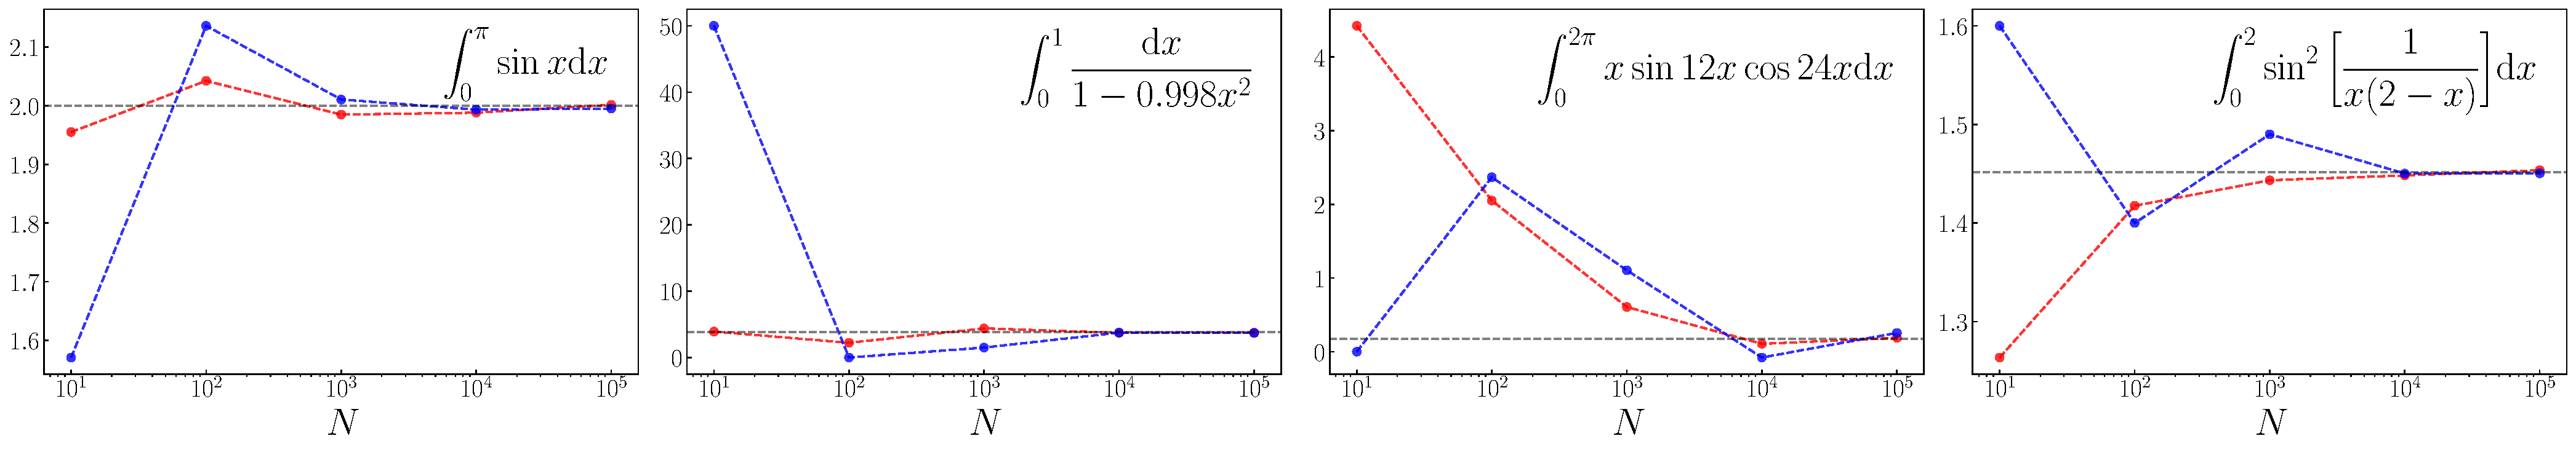
\includegraphics[width=\textwidth]{prob3.pdf}
    \caption{Results for one iteration of rejection (blue) and mean value (red) monte carlo quadrature.}
    \label{fig:prob3}
\end{figure}


\newpage 

\inputpython{prob3.py}

}


\prob{4}{

Compute the following integrals:

\begin{parts}

    \item A double integral over a rectangular region
        \begin{align}
            \int_{0}^{1} \int_{0}^{2} \sin(x^2 + y^2) \dd{x} \dd{y}
        .\end{align}

    \item A double integral over a circular region:
        \begin{align}
            \int_{\rm circle} e^{-(x^2 + y^2)} \dd{x} \dd{y}
        ,\end{align}
        where the circle is centered at the origin with radius $1$.

    \item A double integral over a non-rectangular region
        \begin{align}
            \int_{0}^{1} \int_{0}^{1-x} (x+y) \dd{y} \dd{x}
        .\end{align}

    \item Four-dimensional integral
        \begin{align}
            \int_{0}^{1} \int_{0}^{1} \int_{0}^{1} \int_{0}^{1} \int_{0}^{1} e^{-(x_1^2 + x_2^2 + x_3^2 + x_4^2)} \dd{x_1} \dd{x_2} \dd{x_3} \dd{x_4}
        .\end{align}

    \item Four-dimensional integral over a spherical region
        \begin{align}
            I = \int_{\rm sphere} (x^2 + y^2 + z^2 + w^2) e^{-(x^2 + y^2 + z^2 + w^2)} \dd{x} \dd{y} \dd{z} \dd{w}
        .\end{align}
    
\end{parts}

}


\sol{

(a) The integral here is performed by producing a uniform sample of $N = 10^{6}$ points $(x,y)$ over the rectangular domain $[0,1] \times [0,2]$ and averaging the function values $f(x_{i},y_{i})$, yielding
\begin{align}
    \int_{0}^{1} \dd{x} \int_{0}^{2} \dd{y} \sin(x^2 + y^2) \approx 0.435
.\end{align}


(b) The integral here is performed by uniformly sampling $N = 10^{6}$ points in the circular domain specified by the condition $r = \sqrt{x^2 + y^2} \leq 1$.
This is done by uniformly sampling $(u,\theta) \in [0,1] \times [0,2\pi]$ and computing
\begin{align}
    x &= \sqrt{u} \cos{\theta} \\
    y &= \sqrt{u} \sin{\theta}
.\end{align}
Again, once these samples are produced, we average over the function values, yielding
\begin{align}
    \int_{r \leq 1} e^{-(x^2 + y^2)} \dd{x} \dd{y} \approx 0.632 
.\end{align}


(c) The integral here is performed by producing a uniform sample of $N = 10^{6}$ points $(x,y)$ in the rectangular domain $[0,1]^2$ and writing
\begin{align}
    \int_{0}^{1} \dd{x} \int_{0}^{1 - x} \dd{y} (x + y) = \int_{0}^{1} \dd{x} \int_{0}^{1} \dd{y} (x + y) \Theta(x + y \leq 1)
.\end{align}
Thus, we convert the condition on the integral bounds to one inside the function definition.
Obviously, this is equivalent to rejecting points outside the integration region but upon averaging produces the approximate value
\begin{align}
    \int_{0}^{1} \dd{x} \int_{0}^{1 - x} \dd{y} (x + y) \approx 0.667
.\end{align}


(d) The integral here is performed by producing a uniform sample of $N = 10^{6}$ points $(x_1,x_2,x_3,x_4)$ in the domain $[0,1]^{4}$ and averaging over the function values to obtain
\begin{align}
    \int_{0}^{1} \dd{x_1} \int_{0}^{1} \dd{x_2} \int_{0}^{1} \dd{x_3} \int_{0}^{1} \dd{x_4} e^{-(x_1^2 + x_2^2 + x_3^2 + x_4^2)} \approx 0.311
.\end{align}


(e) The integral here is performed by producing a uniform sample of $N = 10^{6}$ points $(x_1,x_2,x_3,x_4)$ as in the previous part.
From this sample, we excise those points which do not satisfy $r = \sqrt{x_1^2 + x_2^2 + x_3^2 + x_4^2} \leq 1$ and average over the rest to obtain
\begin{align}
    \int_{r \leq 1} \dd{x_1} \dd{x_2} \dd{x_3} \dd{x_4} (x_1^2 + x_2^2 + x_3^2 + x_4^2) e^{-(x_1^2 + x_2^2 + x_3^2 + x_4^2)} \approx 0.316
.\end{align}
While, I did not investigate, there may be a way to generate a uniform sample in ``hyperspherical'' coordinates and transform back to Cartesian coordinates before averaging over function values, allowing one to avoid wasting any samples.

{\color{red} 

It was pointed out that the answers above are incorrect, and upon checking, this statement is true.
In the initial implementation, I forgot to multiply by the area enclosed by the integration domain.
With these amendments, the results are as follows:
\begin{align}
    I_1 &= 0.871 \\
    I_2 &= 1.986 \\
    I_3 &= 0.333 \\
    I_4 &= 0.311 \\
    I_5 &= 1.585
.\end{align}

}


\inputpython{prob4.py}

}

    
\end{document}


